% answers.tex —— 2006 年·普通高等学校招生考试·湖南卷文科 · 参考答案与详细解析片段
% 由 tools/generate_projects.py 依来源总账自 2006/2006_数学真题_湖南文_试题.md + 2006/2006_数学真题_湖南文_解析正文.md + 2006/2006_数学真题_湖南文_答案要点.md 生成，勿手改（改源 MD 后重跑）


\begin{gktip}
以下推导只根据固定候选题面与 Q18 原页图示，为本库非官方草稿。固定 PDF 无答案/解析页；未引用外部答案或评分标准。来源发布者、版次、来源链及官方身份未核。
\end{gktip}

\begin{answer}
\gksolhead{1}{}

\textbf{题目}：

函数 $y=\sqrt{\log_2 x}$ 的定义域是\mbox{（　　）}

\begin{gkopts}(4)
\task （A）$(0,1]$
\task （B）$(0,+\infty)$
\task （C）$(1,+\infty)$
\task （D）$[1,+\infty)$
\end{gkopts}

\Needspace{4\baselineskip}
\textbf{解析}

根号内须非负，故 $\log_2x\geqslant0$；同时 $x>0$。由于底数 $2>1$，两条件合并为 $x\geqslant1$。

\gkanswer{答案：D，$[1,+\infty)$。}

\end{answer}
\begin{answer}
\gksolhead{2}{}

\textbf{题目}：

已知向量 $\vec a=(2,t),\ \vec b=(1,2)$，若 $t=t_1$ 时，$\vec a\parallel\vec b$；$t=t_2$ 时，$\vec a\perp\vec b$，则\mbox{（　　）}

\begin{gkopts}(2)
\task （A）$t_1=-4,\ t_2=-1$
\task （B）$t_1=-4,\ t_2=1$
\task （C）$t_1=4,\ t_2=-1$
\task （D）$t_1=4,\ t_2=1$
\end{gkopts}

\Needspace{4\baselineskip}
\textbf{解析}

平行时行列式 $2\cdot2-t\cdot1=0$，得 $t_1=4$；垂直时点积 $2\cdot1+t\cdot2=0$，得 $t_2=-1$。

\gkanswer{答案：C，$t_1=4,\ t_2=-1$。}

\end{answer}
\begin{answer}
\gksolhead{3}{}

\textbf{题目}：

若 $(ax-1)^5$ 的展开式中 $x^3$ 的系数是 80，则实数 $a$ 的值是\mbox{（　　）}

\begin{gkopts}(4)
\task （A）$-2$
\task （B）$2\sqrt2$
\task （C）$\sqrt[3]{4}$
\task （D）$2$
\end{gkopts}

\Needspace{4\baselineskip}
\textbf{解析}

$(ax-1)^5$ 中 $x^3$ 项来自选出三次 $ax$、两次 $-1$，系数为 $\binom53a^3=10a^3$。令 $10a^3=80$，得 $a^3=8$。

\gkanswer{答案：D，$a=2$。}

\end{answer}
\begin{answer}
\gksolhead{4}{}

\textbf{题目}：

过半径为 2 的球 $O$ 表面上一点 $A$ 作球 $O$ 的截面，若 $OA$ 与该截面所成的角是 $60^\circ$，则该截面的面积是\mbox{（　　）}

\begin{gkopts}(4)
\task （A）$\pi$
\task （B）$2\pi$
\task （C）$3\pi$
\task （D）$2\sqrt3\pi$
\end{gkopts}

\Needspace{4\baselineskip}
\textbf{解析}

球心到截面的距离是 $OA$ 在截面法向上的投影，等于 $2\sin60^\circ=\sqrt3$。截面圆半径 $r$ 满足 $r^2+3=2^2$，故 $r=1$。

\gkanswer{答案：A，$\pi$。}

\end{answer}
\begin{answer}
\gksolhead{5}{}

\textbf{题目}：

“$a=1$”是“函数 $f(x)=|x-a|$ 在区间 $[1,+\infty)$ 上为增函数”的\mbox{（　　）}

\begin{gkopts}(2)
\task （A）充分不必要条件
\task （B）必要不充分条件
\task （C）充要条件
\task （D）既不充分也不必要条件
\end{gkopts}

\Needspace{4\baselineskip}
\textbf{解析}

$|x-a|$ 的折点在 $x=a$。它在 $[1,+\infty)$ 上递增当且仅当 $a\leqslant1$。所以 $a=1$ 足以保证所述增性，但增性也可在 $a<1$ 时成立。

\gkanswer{答案：A，充分不必要条件。}

\end{answer}
\begin{answer}
\gksolhead{6}{}

\textbf{题目}：

在数字 1，2，3 与符号 $+,-$ 五个元素的所有全排列中，任意两个数字都不相邻的全排列个数是\mbox{（　　）}

\begin{gkopts}(4)
\task （A）6
\task （B）12
\task （C）18
\task （D）24
\end{gkopts}

\Needspace{4\baselineskip}
\textbf{解析}

先排两个不同符号，有 $2!$ 种。三个数字不能相邻，必须分别占据符号之间及两端的三个空位；三个数字本身有 $3!$ 种排列。总数为 $2!\cdot3!$。

\gkanswer{答案：B，12。}

\end{answer}
\begin{answer}
\gksolhead{7}{}

\textbf{题目}：

圆 $x^2+y^2-4x-4y-10=0$ 上的点到直线 $x+y-14=0$ 的最大距离与最小距离的差是\mbox{（　　）}

\begin{gkopts}(4)
\task （A）36
\task （B）18
\task （C）$6\sqrt2$
\task （D）$5\sqrt2$
\end{gkopts}

\Needspace{4\baselineskip}
\textbf{解析}

圆心为 $(2,2)$，半径 $r=\sqrt{2^2+2^2+10}=3\sqrt2$。圆心到直线的距离为 $|2+2-14|/\sqrt2=5\sqrt2>r$，直线与圆不相交。圆上到直线的最远、最近距离之差等于圆的直径。

\gkanswer{答案：C，$6\sqrt2$。}

\end{answer}
\begin{answer}
\gksolhead{8}{}

\textbf{题目}：

设点 $P$ 是函数 $f(x)=\sin\omega x$ 的图象 $C$ 的一个对称中心，若点 $P$ 到图象 $C$ 的对称轴上的距离的最小值是 $\dfrac{\pi}{4}$，则 $f(x)$ 的最小正周期是\mbox{（　　）}

\begin{gkopts}(2)
\task （A）$2\pi$
\task （B）$\pi$
\task （C）$\dfrac{\pi}{2}$
\task （D）$\dfrac{\pi}{4}$
\end{gkopts}

\Needspace{4\baselineskip}
\textbf{解析}

设 $\omega\ne0$。$\sin\omega x$ 的对称中心横坐标为 $k\pi/\omega$，竖直对称轴横坐标为 $(\pi/2+j\pi)/\omega$。中心到相邻最近对称轴的距离为 $\pi/(2|\omega|)$；题设使其等于 $\pi/4$，所以 $|\omega|=2$，最小正周期为 $2\pi/|\omega|$。$\omega=0$ 时图象为常值函数，不满足给定的正距离条件。

\gkanswer{答案：B，最小正周期为 $\pi$。}

\end{answer}
\begin{answer}
\gksolhead{9}{}

\textbf{题目}：

过双曲线 $M:x^2-\dfrac{y^2}{b^2}=1$ 的左顶点 $A$ 作斜率为 1 的直线 $l$，若 $l$ 与双曲线 $M$ 的两条渐近线分别相交于点 $B,C$，且 $|AB|=|BC|$，则双曲线 $M$ 的离心率是\mbox{（　　）}

\begin{gkopts}(2)
\task （A）$\dfrac{\sqrt5}{2}$
\task （B）$\dfrac{\sqrt{10}}{3}$
\task （C）$\sqrt5$
\task （D）$\sqrt{10}$
\end{gkopts}

\Needspace{4\baselineskip}
\textbf{解析}

\Needspace{5\baselineskip}
令 $b_0=|b|>0$，渐近线为 $y=\pm b_0x$。取左顶点 $A=(-1,0)$，过 $A$ 的斜率为 $1$ 的直线参数式为 $(x,y)=(-1+t,t)$。它与两渐近线的交点对应参数
\nopagebreak[4]
\[
t_1=\frac{b_0}{b_0-1},\qquad t_2=\frac{b_0}{b_0+1}.
\]
\Needspace{5\baselineskip}
当 $0<b_0<1$ 时两交点分居 $A$ 两侧，$|AB|=|BC|$ 不可能成立；当 $b_0>1$ 时两点同在一侧。较远点到 $A$ 的距离为较近点的两倍，故
\nopagebreak[4]
\[
\frac{b_0}{b_0-1}=2\frac{b_0}{b_0+1},
\]
从而 $b_0=3$。由双曲线标准式，离心率平方为 $1+b_0^2$。

\gkanswer{答案：D，离心率为 $\sqrt{10}$。}

\end{answer}
\begin{answer}
\gksolhead{10}{}

\textbf{题目}：

如图，$OM\parallel AB$，点 $P$ 由射线 $OM$、线段 $OB$ 及 $AB$ 的延长线围成的阴影区域内（不含边界），且 $\overrightarrow{OP}=x\overrightarrow{OA}+y\overrightarrow{OB}$，则实数对 $(x,y)$ 可以是\mbox{（　　）}

\begin{gkopts}(2)
\task （A）$\left(\dfrac14,\dfrac34\right)$
\task （B）$\left(-\dfrac23,\dfrac23\right)$
\task （C）$\left(-\dfrac14,\dfrac34\right)$
\task （D）$\left(-\dfrac15,\dfrac75\right)$
\end{gkopts}
\nopagebreak[4]
\begin{center}% 2006 湖南文科候选卷 Q10；按固定源图的阴影边界重绘，坐标不表示长度比例。
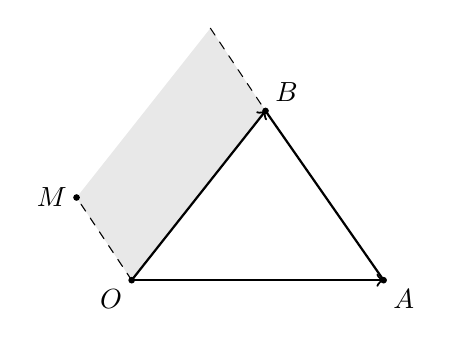
\begin{tikzpicture}[line cap=round,line join=round]
  \coordinate (O) at (0,0);
  \coordinate (A) at (3.2,0);
  \coordinate (B) at (1.7,2.15);
  \coordinate (M) at (-0.7,1.05);
  \coordinate (T) at (1.0,3.2);

  \fill[gray!18] (O)--(M)--(T)--(B)--cycle;

  \draw[dashed] (O)--(M);
  \draw[dashed] (T)--(B);
  \draw[thick] (B)--(A);
  \draw[->,thick] (O)--(B);
  \draw[->,thick] (O)--(A);

  \fill (O) circle[radius=1.2pt];
  \fill (A) circle[radius=1.2pt];
  \fill (B) circle[radius=1.2pt];
  \fill (M) circle[radius=1.2pt];
  \node[below left] at (O) {$O$};
  \node[below right] at (A) {$A$};
  \node[above right] at (B) {$B$};
  \node[left] at (M) {$M$};
\end{tikzpicture}
\end{center}
\nopagebreak[4]
\Needspace{4\baselineskip}
\textbf{解析}

以 $\overrightarrow{OA},\overrightarrow{OB}$ 为平面基底，把 $P$ 表示为 $x\overrightarrow{OA}+y\overrightarrow{OB}$。$AB$ 所在直线满足 $x+y=1$；过 $O$ 且平行于 $AB$ 的射线 $OM$ 在 $x+y=0$ 上。候选 A 满足 $x+y=1$、B 满足 $x+y=0$，都在平行边界上；D 满足 $x+y>1$，在边界外。C 的坐标落在固定 PDF 所示灰色阴影内，故选择 C。此判断按原图所示阴影，不把示意图像素当作精确长度比例。
\nopagebreak[4]
\begin{center}% 2006 湖南文科候选卷 Q10；按固定源图的阴影边界重绘，坐标不表示长度比例。
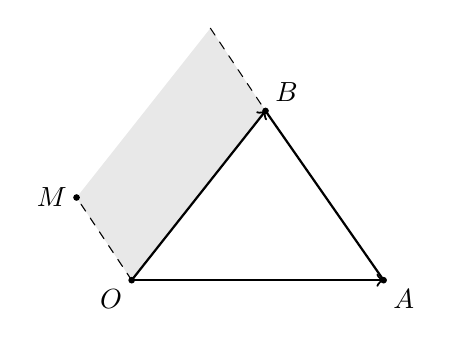
\begin{tikzpicture}[line cap=round,line join=round]
  \coordinate (O) at (0,0);
  \coordinate (A) at (3.2,0);
  \coordinate (B) at (1.7,2.15);
  \coordinate (M) at (-0.7,1.05);
  \coordinate (T) at (1.0,3.2);

  \fill[gray!18] (O)--(M)--(T)--(B)--cycle;

  \draw[dashed] (O)--(M);
  \draw[dashed] (T)--(B);
  \draw[thick] (B)--(A);
  \draw[->,thick] (O)--(B);
  \draw[->,thick] (O)--(A);

  \fill (O) circle[radius=1.2pt];
  \fill (A) circle[radius=1.2pt];
  \fill (B) circle[radius=1.2pt];
  \fill (M) circle[radius=1.2pt];
  \node[below left] at (O) {$O$};
  \node[below right] at (A) {$A$};
  \node[above right] at (B) {$B$};
  \node[left] at (M) {$M$};
\end{tikzpicture}
\end{center}
\nopagebreak[4]
\gkanswer{答案：C，$\left(-\dfrac14,\dfrac34\right)$。}

\end{answer}
\begin{answer}
\gksolhead{11}{}

\textbf{题目}：

若数列 $\{a_n\}$ 满足：$a_1=1,\ a_{n+1}=2a_n,\ n=1,2,3,\ldots$，则 $a_1+a_2+\cdots+a_n=$ \gkblank{}。

\Needspace{4\baselineskip}
\textbf{解析}

\Needspace{5\baselineskip}
递推关系给出等比数列首项 $1$、公比 $2$，第 $n$ 项为 $2^{n-1}$。前 $n$ 项和为
\nopagebreak[4]
\[
1+2+\cdots+2^{n-1}=\frac{2^n-1}{2-1}=2^n-1.
\]

\gkanswer{答案：$2^n-1$。}

\end{answer}
\begin{answer}
\gksolhead{12}{}

\textbf{题目}：

某高校有甲、乙两个数学建模兴趣班。其中甲班 40 人，乙班 50 人。现分析两个班的一次考试成绩，算得甲班的平均成绩是 90 分，乙班的平均成绩是 81 分，则该校数学建模兴趣班的平均成绩是 \gkblank{} 分。

\Needspace{4\baselineskip}
\textbf{解析}

\Needspace{5\baselineskip}
全体学生的平均成绩按人数加权：
\nopagebreak[4]
\[
\frac{40\cdot90+50\cdot81}{40+50}=85.
\]

\gkanswer{答案：85。}

\end{answer}
\begin{answer}
\gksolhead{13}{}

\textbf{题目}：

\Needspace{5\baselineskip}
已知
\nopagebreak[4]
\[
\begin{cases}
x\geqslant1,\\
x-y+1\leqslant0,\\
2x-y-2\leqslant0,
\end{cases}
\]
则 $x^2+y^2$ 的最小值是 \gkblank{}。

\Needspace{4\baselineskip}
\textbf{解析}

约束给出 $x\geqslant1$，$y\geqslant x+1$，$y\geqslant2x-2$。两条关于 $y$ 的下界在 $x=3$ 相交。对 $1\leqslant x\leqslant3$，最小可行 $y=x+1$，函数 $x^2+(x+1)^2$ 随 $x$ 增大；该段最小在 $x=1,y=2$ 处取得。对 $x\geqslant3$，最小可行 $y=2x-2$，$x^2+(2x-2)^2$ 在此段的最小值不小于其 $x=3$ 时的值。故全域最小值在边界点 $(1,2)$ 取得。

\gkanswer{答案：5。}

\end{answer}
\begin{answer}
\gksolhead{14}{}

\textbf{题目}：

过三棱柱 $ABC-A_1B_1C_1$ 的任意两条棱的中点作直线，其中与平面 $ABB_1A_1$ 平行的直线共有 \gkblank{} 条。

\Needspace{4\baselineskip}
\textbf{解析}

作保持直线与平面平行关系的仿射坐标变换，令 $A=(0,0,0)$、$B=(1,0,0)$、$C=(0,1,0)$、$A_1=(0,0,1)$、$B_1=(1,0,1)$、$C_1=(0,1,1)$。平面 $ABB_1A_1$ 为 $y=0$。9 条棱的中点中，有 4 个点的 $y=1/2$；任取其中两个所连的直线均平行于 $y=0$ 的平面，共 $\binom42$ 条。$y=0$ 的中点所连直线落在该平面内，不计为与平面平行；剩余中点只有一个，不能再组成一条平行直线。

\gkanswer{答案：6 条。}

\end{answer}
\begin{answer}
\gksolhead{15}{}

\textbf{题目}：

若 $f(x)=a\sin\left(x+\dfrac{\pi}{4}\right)+3\sin\left(x-\dfrac{\pi}{4}\right)$ 是偶函数，则 $a=$ \gkblank{}。

\Needspace{4\baselineskip}
\textbf{解析}

\Needspace{5\baselineskip}
展开为
\nopagebreak[4]
\[
f(x)=\frac{a+3}{\sqrt2}\sin x+\frac{a-3}{\sqrt2}\cos x.
\]
偶函数的奇函数项系数必须为零，故 $a+3=0$。

\gkanswer{答案：$a=-3$。}

\end{answer}
\begin{answer}
\gksolhead{16}{}

\textbf{题目}：

\Needspace{5\baselineskip}
已知
\nopagebreak[4]
\[
\sqrt3\sin\theta-\frac{\sin\left(\frac{\pi}{2}-2\theta\right)}{\cos(\pi+\theta)}\cdot\cos\theta=1,\qquad \theta\in(0,\pi),
\]
求 $\theta$ 的值。

\Needspace{4\baselineskip}
\textbf{解析}

\Needspace{5\baselineskip}
原式分母要求 $\cos(\pi+\theta)\ne0$，故 $\theta\ne\pi/2$。其余定义域内，利用 $\sin(\pi/2-2\theta)=\cos2\theta$ 及 $\cos(\pi+\theta)=-\cos\theta$，原式化为
\nopagebreak[4]
\[
\sqrt3\sin\theta+\cos2\theta=1.
\]
令 $s=\sin\theta$，并用 $\cos2\theta=1-2s^2$，得 $s(\sqrt3-2s)=0$。由 $\theta\in(0,\pi)$ 可知 $s>0$，只需取非零根。

\gkanswer{答案：$\theta=\dfrac\pi3$ 或 $\dfrac{2\pi}3$。}

\end{answer}
\begin{answer}
\gksolhead{17}{}

\textbf{题目}：

某安全生产监督部门对 5 家小型煤矿进行安全检查（简称安检）。若安检不合格，则必须整改。若整改后经复查仍不合格，则强制关闭。设每家煤矿安检是否合格是相互独立的，且每家煤矿整改前安检是合格的概率是 0.5，整改后安检合格的概率是 0.8，计算（结果精确到 0.01）：

（1） 恰好有两家煤矿必须整改的概率；

（2） 某煤矿不被关闭的概率；

（3） 至少关闭一家煤矿的概率。

\Needspace{4\baselineskip}
\textbf{解析}

\textbf{（1）} 需整改即初检不合格。五家初检独立且各以概率 $1/2$ 不合格，恰有两家不合格的概率为 $\binom52(1/2)^5=0.3125$，按题意精确到百分位。

\textbf{（2）} 单家不被关闭有两种互斥情形：初检通过；或初检未通过而整改复查通过。概率为 $0.5+0.5\cdot0.8=0.90$。

\textbf{（3）} 若各家从初检到复查的结果相互独立，则单家不被关闭的概率为 $0.9$，五家均不被关闭的概率为 $0.9^5$，故至少关闭一家为 $1-0.9^5=0.40951\ldots$，按题意取 $0.41$。但原句只明确“每家煤矿安检是否合格是相互独立的”，未明确跨矿整改复查结果的联合关系；因此 $0.41$ 只是该独立性假设下的条件值，规范答案保留 U/PENDING。

\gkanswer{答案（1）：$0.31$。}

\gkanswer{答案（2）：$0.90$。}

\gkanswer{答案（3）：U/PENDING。}

\end{answer}
\begin{answer}
\gksolhead{18}{}

\textbf{题目}：

如图，已知两个正四棱锥 $P-ABCD$ 与 $Q-ABCD$ 的高都是 2，$AB=4$。

（1） 证明：$PQ\perp$ 平面 $ABCD$；

（2） 求异面直线 $AQ$ 与 $PB$ 所成的角；

（3） 求点 $P$ 到平面 $QAD$ 的距离。
\nopagebreak[4]
\begin{center}% 2006 湖南文科候选卷 Q18；两个共底正四棱锥，按源图结构重绘，不按比例。
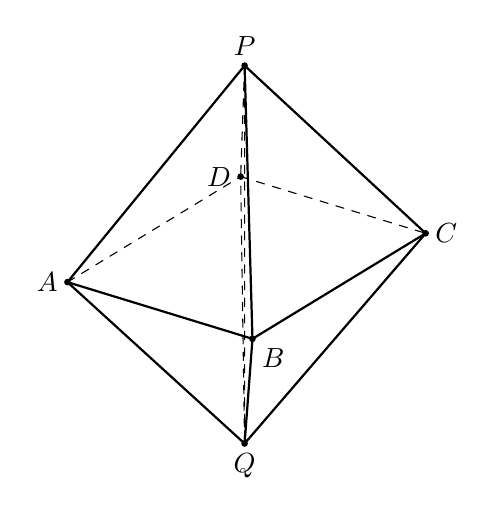
\begin{tikzpicture}[line cap=round,line join=round]
  \coordinate (A) at (-2.2,0);
  \coordinate (B) at (0.15,-0.72);
  \coordinate (C) at (2.35,0.62);
  \coordinate (D) at (0.0,1.34);
  \coordinate (P) at (0.05,2.75);
  \coordinate (Q) at (0.05,-2.05);

  % Hidden back edges and the common altitude line.
  \draw[dashed] (A)--(D) (D)--(C);
  \draw[dashed] (P)--(D) (Q)--(D) (P)--(Q);

  % Visible base and lateral edges.
  \draw[thick] (A)--(B)--(C);
  \draw[thick] (P)--(A) (P)--(B) (P)--(C);
  \draw[thick] (Q)--(A) (Q)--(B) (Q)--(C);

  \foreach \pt in {A,B,C,D,P,Q}{\fill (\pt) circle[radius=1.2pt];}
  \node[left] at (A) {$A$};
  \node[below right] at (B) {$B$};
  \node[right] at (C) {$C$};
  \node[left] at (D) {$D$};
  \node[above] at (P) {$P$};
  \node[below] at (Q) {$Q$};
\end{tikzpicture}
\end{center}
\nopagebreak[4]
\Needspace{4\baselineskip}
\textbf{解析}

\Needspace{5\baselineskip}
按原页示意图，两个正四棱锥顶点位于正方形底面的两侧。取底面中心为原点、底面为 $z=0$，令
\nopagebreak[4]
\[
A=(-2,-2,0),\ B=(2,-2,0),\ C=(2,2,0),\ D=(-2,2,0),\ P=(0,0,2),\ Q=(0,0,-2).
\]
\textbf{（1）} $PQ$ 的方向平行于 $z$ 轴，而底面法向也平行于 $z$ 轴。

\textbf{（2）} 方向向量可取 $\overrightarrow{AQ}=(2,2,-2)$ 与 $\overrightarrow{PB}=(2,-2,-2)$。点积为 $4$，每个向量长度为 $2\sqrt3$；两条直线的锐角余弦为 $1/3$。

\textbf{（3）} 由点 $Q,A,D$ 确定的平面方程为 $x+z+2=0$。将 $P$ 代入点到平面距离公式，分子为 $4$、法向量长度为 $\sqrt2$。
\nopagebreak[4]
\begin{center}% 2006 湖南文科候选卷 Q18；两个共底正四棱锥，按源图结构重绘，不按比例。
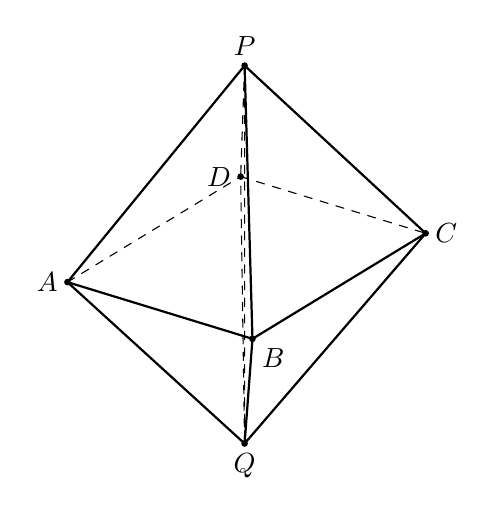
\begin{tikzpicture}[line cap=round,line join=round]
  \coordinate (A) at (-2.2,0);
  \coordinate (B) at (0.15,-0.72);
  \coordinate (C) at (2.35,0.62);
  \coordinate (D) at (0.0,1.34);
  \coordinate (P) at (0.05,2.75);
  \coordinate (Q) at (0.05,-2.05);

  % Hidden back edges and the common altitude line.
  \draw[dashed] (A)--(D) (D)--(C);
  \draw[dashed] (P)--(D) (Q)--(D) (P)--(Q);

  % Visible base and lateral edges.
  \draw[thick] (A)--(B)--(C);
  \draw[thick] (P)--(A) (P)--(B) (P)--(C);
  \draw[thick] (Q)--(A) (Q)--(B) (Q)--(C);

  \foreach \pt in {A,B,C,D,P,Q}{\fill (\pt) circle[radius=1.2pt];}
  \node[left] at (A) {$A$};
  \node[below right] at (B) {$B$};
  \node[right] at (C) {$C$};
  \node[left] at (D) {$D$};
  \node[above] at (P) {$P$};
  \node[below] at (Q) {$Q$};
\end{tikzpicture}
\end{center}
\nopagebreak[4]
\gkanswer{答案（1）：$PQ\perp$ 平面 $ABCD$。}

\gkanswer{答案（2）：$\arccos\dfrac13$。}

\gkanswer{答案（3）：$2\sqrt2$。}

\end{answer}
\begin{answer}
\gksolhead{19}{}

\textbf{题目}：

已知函数 $f(x)=ax^3-3x^2+1-\dfrac3a$。

（1） 讨论函数 $f(x)$ 的单调性；

（2） 若曲线 $y=f(x)$ 上两点 $A,B$ 的切线都与 $y$ 轴垂直，且线段 $AB$ 与 $x$ 轴有公共点，求实数 $a$ 的取值范围。

\Needspace{4\baselineskip}
\textbf{解析}

\Needspace{5\baselineskip}
\textbf{（1）} $a\ne0$，且
\nopagebreak[4]
\[
f'(x)=3x(ax-2).
\]
当 $a>0$，临界点按 $0<2/a$ 排列，导数符号依次为正、负、正；当 $a<0$，临界点次序为 $2/a<0$，导数符号依次为负、正、负。由此得到各开区间上的单调性。

\Needspace{5\baselineskip}
\textbf{（2）} 两条切线垂直于 $y$ 轴，即为水平切线，切点横坐标满足 $f'(x)=0$，为 $0$ 与 $2/a$。其纵坐标分别为
\nopagebreak[4]
\[
f(0)=\frac{a-3}{a},\qquad f(2/a)=\frac{(a-4)(a+1)}{a^2}.
\]
线段与 $x$ 轴有公共点，当且仅当这两个纵坐标乘积不大于零。结合 $a\ne0$，解得参数范围为 $[-1,0)\cup[3,4]$。

\gkanswer{答案（1）：当 $a>0$ 时，递增区间为 $(-\infty,0)$、$(2/a,+\infty)$，递减区间为 $(0,2/a)$；当 $a<0$ 时，递减区间为 $(-\infty,2/a)$、$(0,+\infty)$，递增区间为 $(2/a,0)$；$a=0$ 不在定义域内。}

\gkanswer{答案（2）：$a\in[-1,0)\cup[3,4]$。}

\end{answer}
\begin{answer}
\gksolhead{20}{}

\textbf{题目}：

在 $m\ (m\geqslant2)$ 个不同数的排列 $P_1P_2\cdots P_m$ 中，若 $1\leqslant i\leqslant j\leqslant m$ 时 $P_i>P_j$（即前面某数大于后面某数），则称 $P_i$ 与 $P_j$ 构成一个逆序。一个排列的全部逆序的总数称为该排列的逆序数。记排列 $(n+1)n(n-1)\cdots321$ 的逆序数为 $a_n$，如排列 21 的逆序数 $a_1=1$，排列 321 的逆序数 $a_2=3$，排列 4321 的逆序数 $a_3=6$。

（1） 求 $a_4,a_5$，并写出 $a_n$ 的表达式；

（2） 令 $b_n=\dfrac{a_n}{a_{n+1}}+\dfrac{a_{n+1}}{a_n}$，证明：$2n<b_1+b_2+\cdots+b_n<2n+3,\ n=1,2,\ldots$。

\begin{gktip}
Q20 的条件在固定原页中印作 $1\leqslant i\leqslant j\leqslant m$，本稿按原样转录，未据定义或题意改写。
\end{gktip}

\Needspace{4\baselineskip}
\textbf{解析}

\textbf{（1）} 降序排列 $(n+1)n\cdots321$ 中每一对数都构成逆序，故逆序数为 $\binom{n+1}{2}$。印刷条件含 $i=j$，但各数互异时 $P_i>P_i$ 不成立；按原文求逆序不会额外计入对角项。

\Needspace{5\baselineskip}
\textbf{（2）} 令 $b_n=a_n/a_{n+1}+a_{n+1}/a_n$，代入 $a_n=n(n+1)/2$ 得
\nopagebreak[4]
\[
b_n=\frac{n}{n+2}+\frac{n+2}{n}=2+\frac4{n(n+2)}=2+2\left(\frac1n-\frac1{n+2}\right).
\]
求和后为 $2n+3-2/(n+1)-2/(n+2)$。后两项之和大于 $0$，且小于 $3$，从而满足所要求的严格上下界。

\gkanswer{答案（1）：$a_4=10,\ a_5=15,\ a_n=\dfrac{n(n+1)}2$。}

\gkanswer{答案（2）：$b_n=2+\dfrac4{n(n+2)}$，$b_1+b_2+\cdots+b_n=2n+3-\dfrac2{n+1}-\dfrac2{n+2}$。}

\end{answer}
\begin{answer}
\gksolhead{21}{}

\textbf{题目}：

已知椭圆 $C_1:\dfrac{x^2}{4}+\dfrac{y^2}{3}=1$，抛物线 $C_2:(y-m)^2=2px\ (p>0)$，且 $C_1,C_2$ 的公共弦 $AB$ 过椭圆 $C_1$ 的右焦点。

（1） 当 $AB\perp x$ 轴时，求 $m,p$ 的值，并判断抛物线 $C_2$ 的焦点是否在直线 $AB$ 上；

（2） 若 $p=\dfrac43$ 且抛物线 $C_2$ 的焦点在直线 $AB$ 上，求 $m$ 的值及直线 $AB$ 的方程。

\par\medskip

\begin{gktip}
\textbf{来源说明}：题面据来源总账登记的固定候选 PDF 转录；文件 SHA-256 与 Git blob 见 \texttt{source-manifest.json}，逐题页码和来源指纹见本卷 \texttt{provenance.json}。发布者、版次、来源链及官方身份未核；固定 PDF 不含答案或解析。
\end{gktip}

\Needspace{4\baselineskip}
\textbf{解析}

椭圆半焦距 $c=\sqrt{4-3}=1$，右焦点为 $F=(1,0)$。

\Needspace{5\baselineskip}
\textbf{（1）} 若公共弦垂直于 $x$ 轴，则其直线为 $x=1$。与椭圆的交点为 $(1,\pm3/2)$。两点同时在抛物线上要求
\nopagebreak[4]
\[
\left(\frac32-m\right)^2=\left(-\frac32-m\right)^2,
\]
故 $m=0$；代回抛物线方程得 $p=9/8$。该抛物线焦点横坐标为 $p/2=9/16$，不等于弦所在直线的横坐标。

\textbf{（2）} 此时抛物线焦点为 $G=(2/3,m)$。若弦 $AB$ 经过 $F,G$，其直线方程为 $y=-3m(x-1)$。将该式分别代入椭圆和抛物线方程，可得关于 $x$ 的二次式。两曲线的弦端点相同，要求两二次式成比例；比较常数项与二次项系数之比，得 $m^2=2/3$。代回检验一次项系数也满足相同比例，且所得两根互异。因此 $m=\pm\sqrt6/3$，相应直线为 $y=-3m(x-1)$。

\gkanswer{答案（1）：$m=0,\ p=\dfrac98$；抛物线焦点为 $(\dfrac9{16},0)$，不在 $AB:x=1$ 上。}

\gkanswer{答案（2）：$m=\pm\dfrac{\sqrt6}{3}$；对应 $AB$ 方程为 $y=-3m(x-1)$。}

\end{answer}